In the accompanying figure, the outer square has side length 40. A second square S' of side length 15 is constructed inside S with the same center as S and with sides parallel to those of S. From each midpoint of a side of S, segments are drawn to the two closest vertices of S'. The result is a four-pointed starlike figure inscribed in S. The star figure is cut out and then folded to form a pyramid with base S'. Find the volume of this pyramid.
\begin{center}
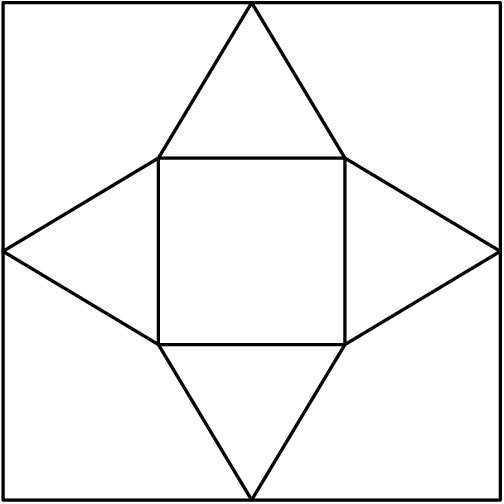
\includegraphics[width = 50.400000000000006mm]{img/fig0.png}
\end{center}